\documentclass[10pt,twocolumn]{article}

% use the oxycomps style file
\usepackage{oxycomps}

% usage: \fixme[comments describing issue]{text to be fixed}
% define \fixme as not doing anything special
\newcommand{\fixme}[2][]{#2}
% overwrite it so it shows up as red
\renewcommand{\fixme}[2][]{\textcolor{red}{#2}}
% overwrite it again so related text shows as footnotes
%\renewcommand{\fixme}[2][]{\textcolor{red}{#2\footnote{#1}}}

% read references.bib for the bibtex data
\bibliography{references}

% include metadata in the generated pdf file
\pdfinfo{
    /Title (Git and LaTeX Worksheet)
    /Author (Justin Li)
}

% set the title and author information
\title{Git and \LaTeX Worksheet}
\author{Justin Li}
\affiliation{Occidental College}
\email{justinnhli@oxy.edu}

\begin{document}

\maketitle

\section{Instructions}

This worksheet is due March 1, 2025 at midnight, to be submitted as a GitHub repository URL to Canvas. The repository should contain all files requires to compile this worksheet with your answers. You should only change this \texttt{document.tex} file and the  \texttt{references.bib} file; do not change any other file in this starting repository. You should not use any additional packages, and are not allowed to use the \texttt{{\textbackslash}usepackage\{\}} command. Additionally, the output should be formatted correctly: your answers should be appropriately nested under the questions, command-line commands should be in monospace, and images should be positioned appropriately.

\section{Git Questions}

\subsection{General questions}

\begin{enumerate}
    \item What is a version control system? Why are they useful?
        \begin{itemize}
            \item A version control system manages various iterations of files / projects. They allow collaboration, returns to previous versions, and a history of changes.
        \end{itemize}
    \item What is the difference between git and GitHub?
        \begin{itemize}
            \item git is the version control software, while GitHub is a hosting service that uses the software git.
        \end{itemize}
    \item What is a repository?
        \begin{itemize}
            \item A repository is a collection of files (like a folder / directory).
        \end{itemize}
    \item What is a commit?
        \begin{itemize}
            \item A commit is a set of changes to a repository. It can be thought of as a moment in the history of a repository.
        \end{itemize}
    \item What is the commit graph?
        \begin{itemize}
            \item The commit graph illustrates the commit history of a repository, including important information such as the branches.
        \end{itemize}
    \item What is your preferred local git client (eg., command line, GitHub Desktop, GitKraken, etc.)?
        \begin{itemize}
            \item I have been using a combination of command line, GitHub Desktop, GitKraken, and my IDE (VSCode); it depends on what I am trying to do. If I'm merging or rebasing, I use command line. If I'm just commiting, I use GitHub Desktop or VSCode. If I want to see the commit graph, I use GitKraken.
        \end{itemize}
\end{enumerate}

\subsection{Local Usage}

\begin{enumerate}
    \item What is the difference between adding a file to the staging area and committing a file?
        \begin{itemize}
            \item Adding a file to the staging area means it is ready to be included in a commit, while committing a file means it has actually been added to the history of the repository.
        \end{itemize}
    \item What is a commit message, and why is it important for them to be meaningful?
        \begin{itemize}
            \item A commit message details what changes were made in the commit, or in other words, why the commit was made. It is important for it to be meaningful so that you or another person can look back and understand what was done.
        \end{itemize}
    \item Starting with an empty repository, what sequence of commands/actions would result in the following commit graph? You may give a sequence of \texttt{git} commands, or describe (with screenshots) how you would do this in your preferred graphical git interface.
        \begin{verbatim}
        A---B---C---D
        \end{verbatim}
        \begin{itemize}
            \item Assuming the letter of each commit is the commit message, and there are changes in the staging area in between each commit...
            \item \texttt{git commit -m A}
            \item \texttt{git commit -m B}
            \item \texttt{git commit -m C}
            \item \texttt{git commit -m D}
        \end{itemize}
    \item If you are currently at commit D above, how would you recover code from commit B? What sequence of commands/actions would let you do so? You may give a sequence of \texttt{git} command-line commands, or describe (with screenshots) how you would do this in your preferred graphical git interface. Assume the commit hashes are AAAAAA..., BBBBBB..., etc.
        \begin{itemize}
            \item \texttt{git checkout BBBBBB}
        \end{itemize}
    \item Imagine you created a git repository for your project, but only commit your changes once a week on Sundays. You got your code working on Tuesday, but then broke your code on Friday. What can you do to get the working version of your code back?
        \begin{itemize}
            \item You can't, unless you stored the working code somewhere else. It is not accessible from git since no commit was made.
        \end{itemize}
\end{enumerate}

\subsection{Branching and Merging}

\begin{enumerate}
    \item What is a branch? Why are they useful?
        \begin{itemize}
            \item A branch is a tag associated with commits which creates an independent line of development.
        \end{itemize}
    \item Starting with an empty repository, what sequence of commands/actions would result in the following commit graph? You may give a sequence of \texttt{git} command-line commands, or describe (with screenshots) how you would do this in your preferred graphical git interface.
        \begin{verbatim}
        A---B---C---D
             \
              E---F
        \end{verbatim}
        \begin{itemize}
            \item \texttt{git commit -m A}
            \item \texttt{git commit -m B}
            \item \texttt{git checkout -b new\_branch}
            \item \texttt{git commit -m E}
            \item \texttt{git commit -m F}
            \item \texttt{git checkout main}
            \item \texttt{git commit -m C}
            \item \texttt{git commit -m D}
        \end{itemize}
    \item Why is a merge? Why are they useful?
        \begin{itemize}
            \item A merge combines the changes of two commits. They allow for the integration of different branches.
        \end{itemize}
    \item Imagine you are currently at commit D above. What sequence of commands/actions would result in the following commit graph? You may give a sequence of \texttt{git} commands, or describe (with screenshots) how you would do this in your preferred graphical git interface.
        \begin{verbatim}
        A---B---C---D---G
             \         /
              E---F---/
        \end{verbatim}
        \begin{itemize}
            \item \texttt{git merge new\_branch}
        \end{itemize}
    \item What is a merge conflict? When do they occur?
        \begin{itemize}
            \item A merge conflict is when a merge is attempting to combine changes (i.e. the same line of a file, deleting a file with edits, two files with same name), such that the system is unable to clearly accept both.
        \end{itemize}
    \item Starting with an empty repository, despite a sequence of commands/actions that would result in a merge conflict. Include the exact edits and \texttt{git} commands or screenshots of the graphical git interface. Include the output or screenshot that shows the resulting merge conflict.
        \begin{itemize}
            \item \texttt{git init}
            \item \texttt{touch file.py}
            \item \texttt{vim file.py}
            \item 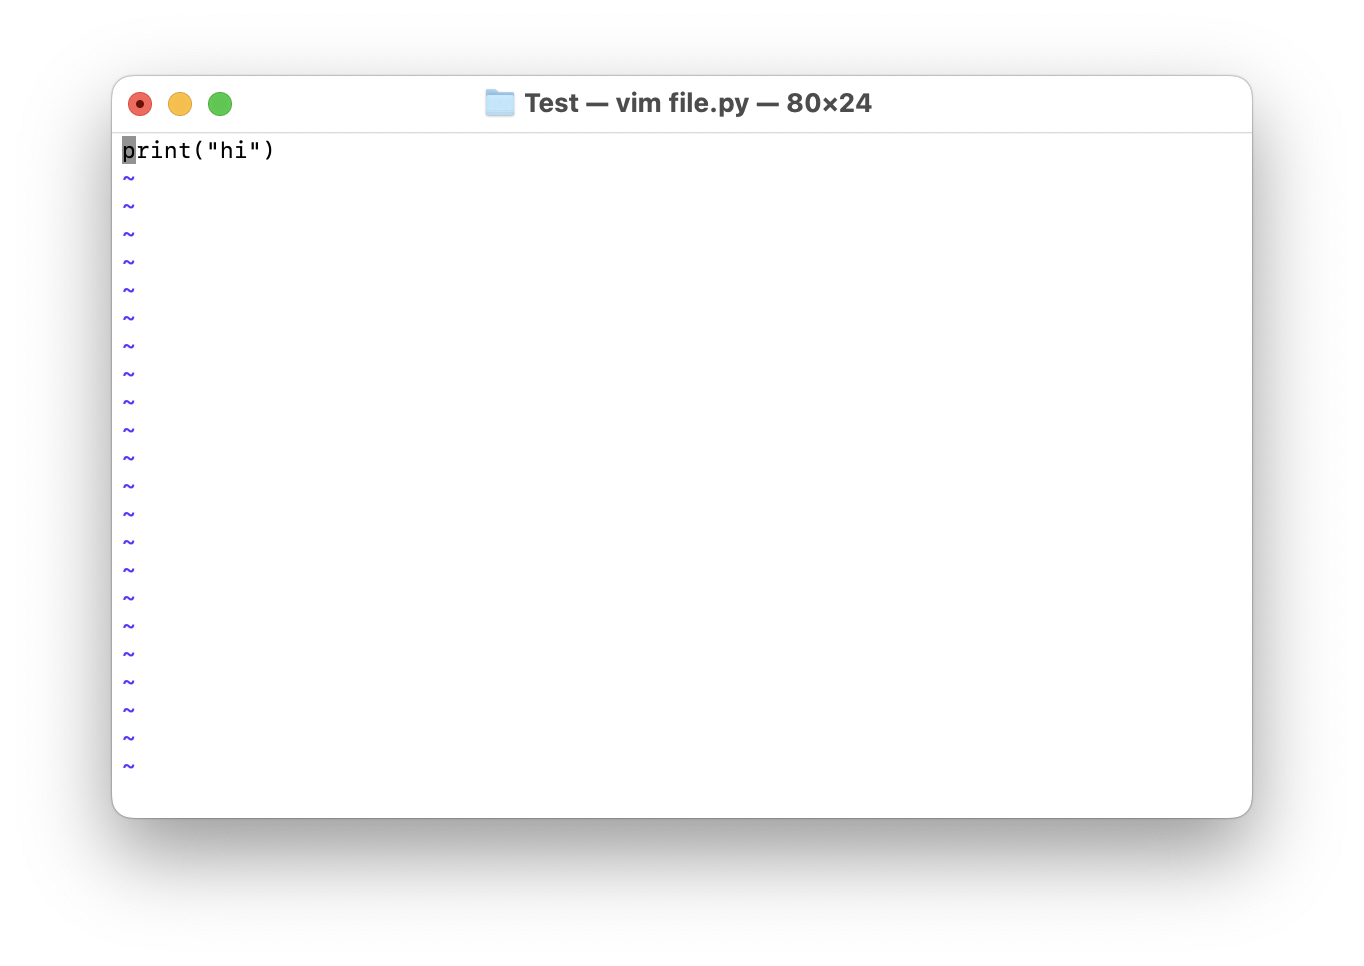
\includegraphics[width=0.5\linewidth]{Images/1.png}
            \item \texttt{git add file.py}
            \item \texttt{git commit -m A}
            \item \texttt{git branch -b new\_branch}
            \item \texttt{vim file.py}
            \item 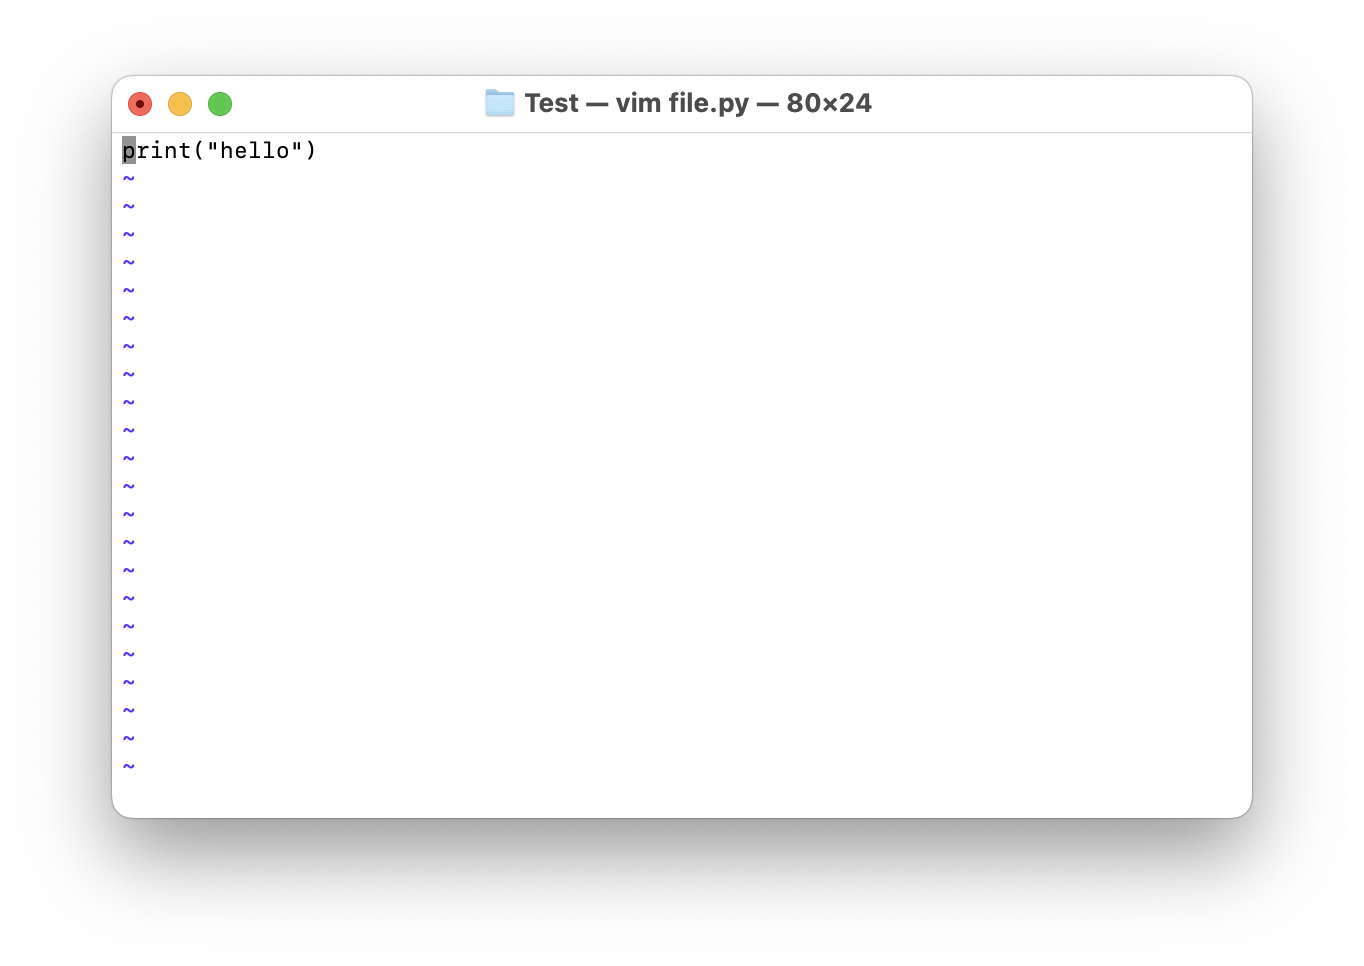
\includegraphics[width=0.5\linewidth]{Images/2.png}
            \item \texttt{git add file.py}
            \item \texttt{git commit -m "Print hello"}
            \item \texttt{git checkout main}
            \item \texttt{vim file.py}
            \item 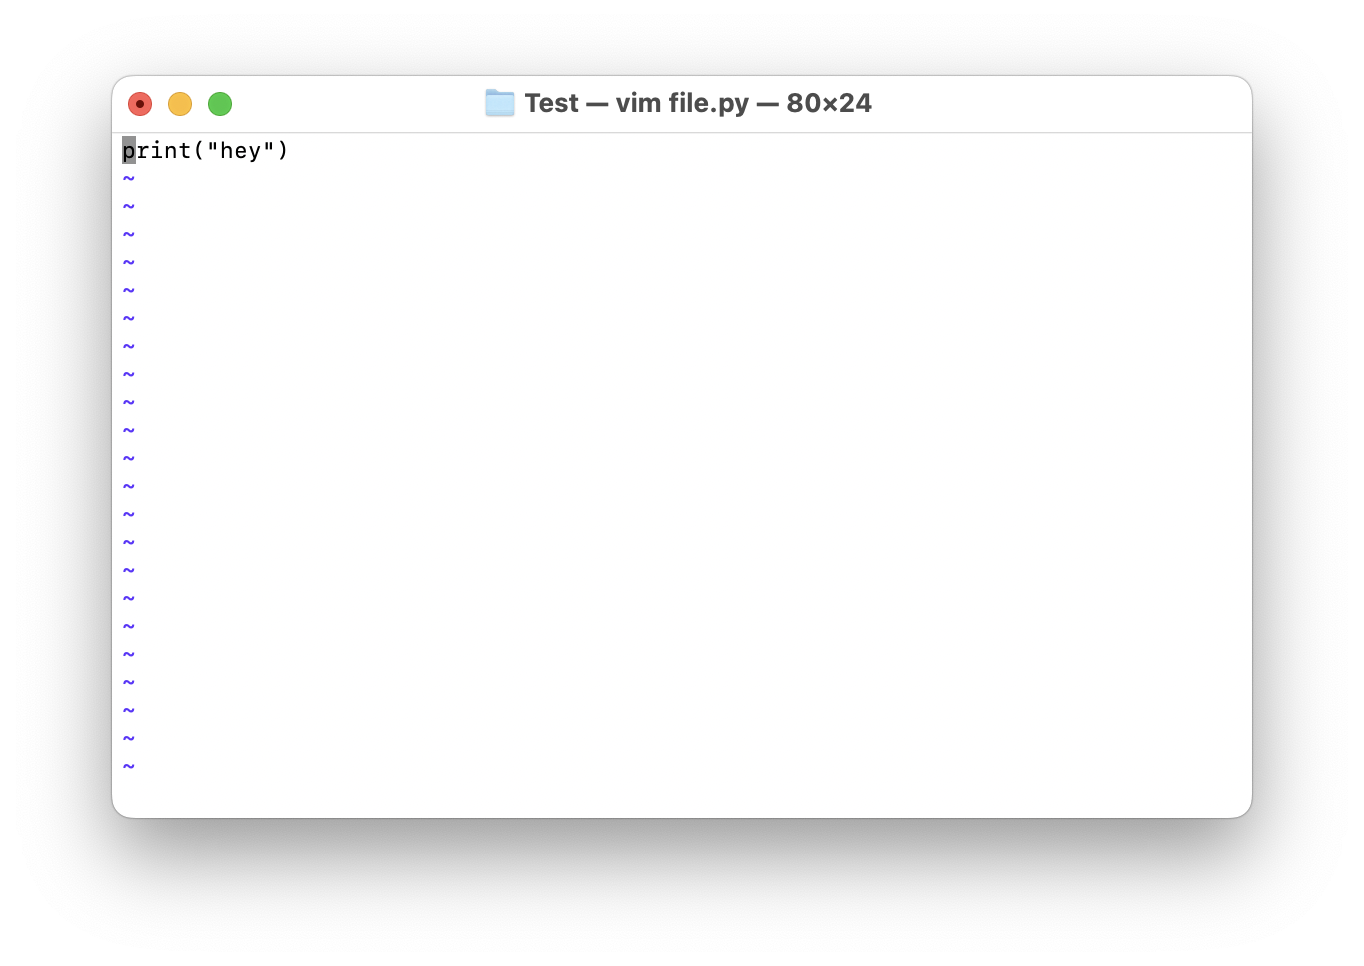
\includegraphics[width=0.5\linewidth]{Images/3.png}
            \item \texttt{git add file.py}
            \item \texttt{git commit -m "Print hey"}
            \item \texttt{git merge new\_branch}
            \item 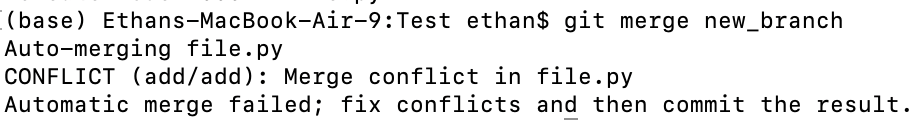
\includegraphics[width=0.5\linewidth]{Images/4.png}
        \end{itemize}
\end{enumerate}

\subsection{Remotes}

\begin{enumerate}
    \item What is a remote?
        \begin{itemize}
            \item A remote is an online repository that may be accessible from different devices. This is one of the big advantages of a service like GitHub.
        \end{itemize}
    \item What does pushing and pulling do?
        \begin{itemize}
            \item Pushing sends your local repository to the remote repository. Pulling downloads any updates from the remote repository to the local repository.
        \end{itemize}
    \item Imagine you created a git repository for your project on your laptop and commit regularly, but only push your code to GitHub once a week on Sundays. Your laptop caught on fire on Friday. What can you do to get your code back?
        \begin{itemize}
            \item You can't recover any updates made from that week (in the time since the last push). You can only get the Sunday commit back.
        \end{itemize}
\end{enumerate}

\section{\LaTeX}

Find a source of each of the following types and add it to \texttt{references.bib}, with the appropriate data. Your sources do not have to relate to your project. Looking at \textcite{OverleafBibliographyManagement} and \textcite{WikipediaBibtex} may be helpful,

\begin{itemize}
    \item a journal article \cite{Journal}
    \item a conference article \cite{Conference}
    \item a PhD or Master's thesis \cite{PhD}
    \item an article in an edited popular media venue (newspaper, magazine, etc.) \cite{Magazine}
    \item a book \cite{Book}
    \item a chapter of a book \cite{Chapter}
    \item a YouTube video \cite{Video}
    \item a piece of technical documentation (e.g., a programming language reference, and API documentation, etc.) \cite{Documentation}
\end{itemize}

Additionally, in you own words, explain the difference between \texttt{{\textbackslash}cite\{\}} and \texttt{{\textbackslash}textcite\{\}}. When should they each be used? Demonstrate your answers by using one of them with each of your references from above.
    \begin{itemize}
        \item \texttt{{\textbackslash}cite\{\}} only puts a numerical citation at the end of the sentence, and should be used when the citation should not be in the text. \texttt{{\textbackslash}textcite\{\}} is a textual citation that should be used when the author should be part of the text / sentence.
        \item Computer Science can be "taught" in less than 20 minutes \cite{Video}.
        \item \textcite{Magazine} details how an undergraduate student improved hash tables.
    \end{itemize}

\printbibliography

\end{document}
